\section{Theorie}
\label{sec:theorie}

\subsection{Das Standardmodell der Teilchenphysik}

Der Aufbau der Materie sowie die Wechselwirkungen dieser auf elementarer Ebene werden durch das so
genannte Standardmodell der Teilchenphysik beschrieben. Dieses Modell enthält alle bisher bekannten
Elementarteilchen und beschreibt abgesehen von der Gravitation die Mechanismen ihrer Wechselwirkungen
untereinander. Dabei lassen sich die Teilchen anhand ihrer Eigenschaften in verschiedene Gruppen aufteilen.
Die Fermionen (also Spin-$\sfrac{1}{2}$-Teilchen, welche der Fermi-Dirac-Statistik gehorchen) gliedern sich in
Leptonen und Quarks. Letztere nehmen an der starken Wechselwirkung teil, welche über die Gluonen vermittelt wird.
Diese sind Spin-1-Bosonen. Die Quarks bilden außerdem durch Bindung die Hadronen wie etwa Protonen, Neutronen etc. sowie ihre Antiteilchen. Die
Leptonen nehmen ledigich an der elektroschwachen Wechselwirkung teil, welche über Photonen (ebenfalls
Spin-1-Bosonen), sowie das $Z^0$-Boson und die $W^{\pm}$-Bosonen wirkt. Sie gliedern sich in 3 Generationen: Die Elektron-, die Myon- sowie die Tauon-Generation. Die einzelnen Generationen bestehen aus dem geladenen Lepton und dem neutralen Neutrino, sowie ihren Antiteilchen. Zusammen mit dem Higgs-Boson und den
zugehörigen Antiteilchen (wobei das Photon sein eigenes Antiteilchen ist) ergibt sich die
in Abbildung~\ref{fig:sm} dargestellte Menge der Elementarteilchen.
%
\begin{figure}[htb]
  \centering
  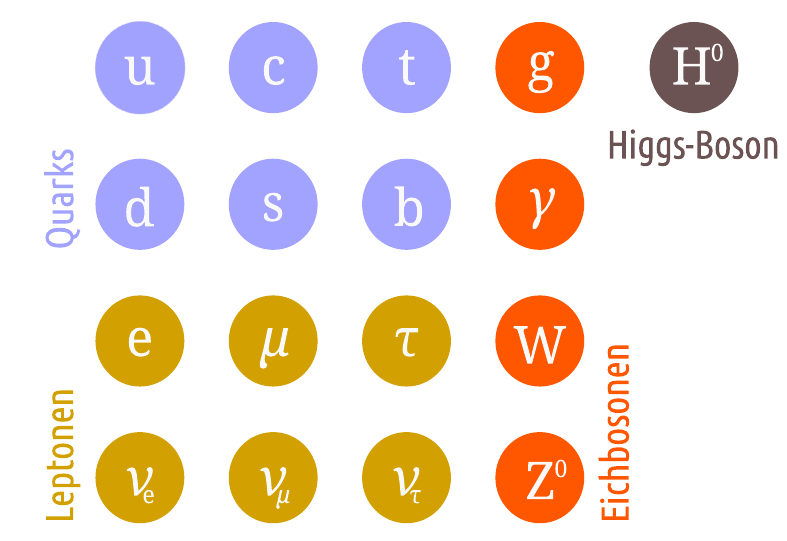
\includegraphics[width=0.6\textwidth]{figures/standardmodell.png}
  \caption{Übersicht der Elementarteilchen im Standardmodell.}
  \label{fig:sm}
\end{figure}
%
Die in diesem Versuch untersuchten Myonen entstehen in der oberen Atmosphäre aus Zerfällen von Pionen.
%
\begin{align}
  \pi^+\rightarrow\mu^++\nu_\mu \\
  \pi^-\rightarrow\mu^-+\bar{\nu}_\mu
\end{align}
%
Aufgrund ihrer hohen kinetischen Energie gelangen die Myonen trotz hrer kurzen Lebensdauer zu einem großen Teil bis zur
Erdoberfläche. Dort können sie über Szintillationsdetektoren nachgewiesen werden. Dabei geben sie beim Durchqueren eines
Szintillatormaterials mehrere MeV Energie an dieses Material ab. Diese Energie regt das Szintillatormaterial an, sodass dieses beim Abregen ein Photon emittiert, welches detektiert wird.
Gibt ein Myon seine gesamte kinetische Energie im Szintillatormaterial ab, so zerfällt dieses anschließend auch dort. Die Zerfälle, die hier möglich sind, sind die folgenden:
%
\begin{align}
  \mu^\pm\rightarrow e^\pm\nu_\mu \\
\end{align}
%
Dabei entstehen hochenergetische Elektronen bzw. Positronen, da das Myon rund 200mal schwerer ist, als diese Teilchen.
Die entstandenen Teilchen erzeugen wiederum Lichtblitze. Die Zeit zwischen diesen Impulsen entspricht der Lebensdauer
des Myons im Detektor. Da hochenergetische Myonen nicht im Detektor zerfallen, allerdings beim Eindringen trotzdem einen
Lichtblitz auslösen und somit einen Startimpuls für eine Messung, muss experimentell sichergestellt werden, dass diese
Signale nicht in den Ergebnissen gespeichert werden.
%
\subsection{Bestimmung der mittleren Lebensdauer von Elementarteilchen}

In diesem Versuch werden, wie in der Zielsetzung bereits erwähnt, Individuallebensdauern gemessen. Die tatsächliche Zeit
von der Entstehung eines Myons bis zum Zerfall desselben stellt allerdings eine statistisch verteilte Größe dar, weil es
sich bei dem Prozess um einen zufällig auftretenden Prozess handelt. Jeder Prozess ist dabei von anderen Zerfällen
unabhängig. Es ist daher notwendig den Begriff der mittleren Lebensdauer bestimmter Teilchenarten verallgemeinert zu definieren.
Dazu wird die Tatsache genutzt, dass die infinitessimale Wahrscheinlichkeit $\upd W$ für einen Zerfall proportional zum
betrachteten infinitessimalen Zeitintervall $\upd t$ ist:
%
\begin{equation}
  \upd W=\lambda\upd t \; .
\end{equation}
%
Die Proportionalität wird hierbei durch $\lambda$ beschrieben. Hieraus wird ebenfalls ersichtlich, dass sie nicht explizit von einem Zeitpunkt $t$ abhängig ist. Aus der Unabhängigkeit
der einzelnen Zerfälle folgt die infinitessimale Anzahl der Zerfälle im Intervall $\upd t$ als
%
\begin{equation}
  \upd N=-N\upd W=-\lambda N\upd t \; .
\end{equation}
%
Wird nun eine sehr große Anzahl an Zerfällen betrachtet, lässt sich dieser Zusammenhang als kontinuierlich nähern und
integrieren. Es folgt ein Zusammenhang, welcher die Anzahl der Zerfälle nach einer Zeit $t$ aus anfänglich $N_0$
Teilchen angibt.
%
\begin{equation}
  N(t)=N_0\exp(-\lambda t)
\end{equation}
%
Hieraus lässt sich die Anzahl $\upd N$ der Zerfälle in einem Zeitintervall $\upd t$ aus
%
\begin{equation}
  \frac{\upd N}{N_0}=\frac{N(t)-N(t+\upd t)}{N_0}
\end{equation}
%
berechnen. Diese Verteilungsfunktion lautet:
%
\begin{equation}
  \frac{\upd N(t)}{N_0}=\lambda\exp(-\lambda t)\upd t
\end{equation}
%
Durch Bilden des Mittelwertes der verschiedenen Häufigkeiten mit deren Wahrscheinlichkeit gewichtet entsteht so der
Erwartungswert der mittleren Lebensdauer. Dieser Erwartungswert ist allgemein als
%
\begin{equation}
  \symup{E}x:=\int_{-\infty}^{\infty}xf(x)\upd x
\end{equation}
%
definiert. In dem betrachteten Zerfall ergibt sich so für die verallgemeinerte Lebensdauer $\tau$
%
\begin{equation}
  \tau=\symup{E}T=\int_0^\infty t\lambda\exp(-\lambda t)\upd t=\left[\lambda\left(-\frac{t}{\lambda}-\frac{1}{\lambda^2}\right)\exp(-\lambda t)\right]^\infty_0=\frac{1}{\lambda} \; .
\end{equation}
%
In diesem Zusammenhang wird $\lambda$ als Zerfallskonstante bezeichnet.
